\documentclass[11pt]{article}
\usepackage{graphicx} % Required for inserting images
\usepackage[top=2.5cm, bottom=2.5cm, left=2.5cm, right=2.5cm]{geometry}
\usepackage[T1]{fontenc}
\usepackage{hyperref}
\usepackage[utf8]{inputenc}
\usepackage{multirow}
\usepackage{subcaption}
\usepackage{booktabs}
\usepackage{bookmark}
\usepackage{graphicx}
\usepackage{setspace}
\setlength{\parindent}{0in}
\usepackage{physics}
\usepackage{tikz}
\usepackage{tikz-3dplot}
\usepackage[outline]{contour} % glow around text
\usepackage{xcolor}
\usepackage{float}
\usepackage{makeidx}
\usepackage{fancyhdr}
\usepackage{pgfplots}
\usepackage{amsmath}
\pgfplotsset{compat=1.18}
\usepackage{caption}
\usepackage[english,catalan]{babel}
\setlength{\parskip}{11pt}
\usepackage{xcolor}
\usepackage{listings}
\usepackage{marginnote}

\title{\Huge\bfseries Pràctica de simulació: \\ Instal·lació de panells solars fotovoltaics en un habitatge unifamiliar a Catalunya \\ [2ex] \Large}

\author{\begin{tabular}{c}
\textbf{GRUP C3} \\
Isaac Baldi García (1667260)\\
Marcel López Freixes (1668323) \\
Eira Jacas García (1666616) \\
Núria Castillo Ariño (1669145)
\end{tabular}}

\date{07/1/01/2025}

\begin{document}

\maketitle

Abstract pràctica 

\section{Moviment de la Terra al voltant del Sol} \label{sec: seccio_1}
En aquesta secció ens hem proposat simular el moviment de translació de la Terra al voltant del Sol. Per fer-ho hem partit de la Llei de la Gravitació Univeral i hem simplificant el nostre problema de dos cossos a un d'un sol cos sota una força central, $F(r)$.
\begin{equation}
    F(r)=-\frac{GMm}{r^2}
\end{equation}

On G és la constant de grabitació universal, M la massa del Sol i m la massa de la Terra.\footnote{Totes les dades orbitalàries agafades del Jet Propulsion Laboratory de la NASA: \url{https://ssd.jpl.nasa.gov/}}

Per aquest tipus de sistemes i considerant únicament aquesta força central, tenim dues equacions de moviment en el pla polar 
\begin{equation}
    F(r)=m\ddot{r}-mr{\dot{\theta}}^2
    \label{equ_en_r}
\end{equation}
\begin{equation}
    0=\ddot{\theta}m=mr\ddot{\theta}+2m\dot{r}\dot{\theta}
    \label{equ_en_theta}
\end{equation}
i la propietat que el moment angular es conserva
\begin{equation}
    L=mr\dot{\theta}=ctt
    \label{moment_angular}
\end{equation}

Combinant les equacions \eqref{equ_en_r} i \eqref{moment_angular} obtenim una EDO que només depen de r i una EDO que només depen de $\theta$
\begin{equation}
    \frac{\partial\dot{r}}{\partial t}=-GM\frac{1}{r^2}+\frac{L^2}{m^2r^3}
    \label{edor}
\end{equation}
\begin{equation}
    \frac{\partial}{}
    \label{edot}
\end{equation}
Normalitzant aquestes dues equacions i reduint l'ordre de l'equació \eqref{edor} obtenim
\begin{equation}
    \frac{\partial\tilde{v}}{\partial\tilde{t}}=-\frac{1}{\tilde{r}^2}+\frac{1}{\tilde{r}^3}
    \label{1_edo_r}
\end{equation}
\begin{equation}
    \frac{\partial\tilde{r}}{\partial\tilde{t}}=\tilde{v}
    \label{2_edo_r}
\end{equation}
\begin{equation}
    \frac{\partial\tilde{\theta}}{\partial\tilde{t}}=\frac{1}{\tilde{r}^2}
    \label{edo_tetha}
\end{equation}
on les variables normalitzades segueixen $r=\tilde{r}\alpha$, $t=\tilde{t}\frac{\alpha}{\bar{v}}$, $v=\tilde{v}\bar{v}$ i les constants de normalització $\alpha = \frac{\beta}{\kappa}$, $\bar{v}=\frac{\kappa}{(\beta)^{1/2}}$, $\beta=\frac{L^2}{m^2}, \kappa=GM$.

Aquest sistema d'equacions diferencials de primer ordre l'hem resolt numèricament amb el mètode d'Euler i agafant com a condicions de contorn el radi de l'òrbita, la velocitat radial i l'angle al periheli.\footnotemark[\value{footnote}]
Si grafiquem els resultats obtenim
\begin{figure}[h]
    \centering
    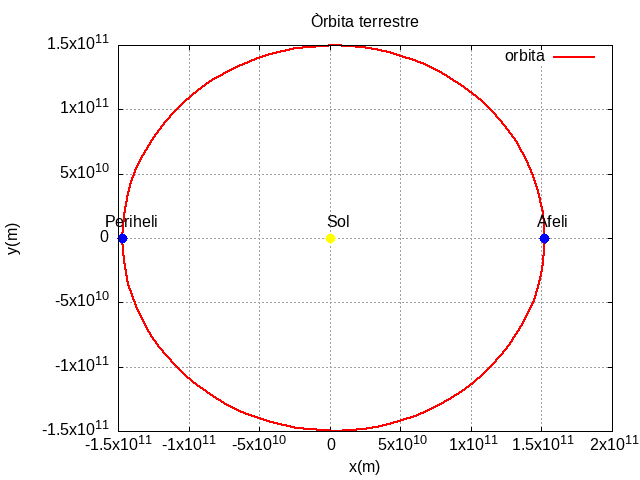
\includegraphics[width=0.5\textwidth]{orbita.png}
    \label{orb_terra}
    \caption{Òrbita Terrestre calculada numèricament}
\end{figure}

El mètode d'Euler és poc exacte però amb una discretització prou fina dona bons resultats. Si calculem l'error acomulat en el radi al completar una Òrbita sencera amb una discretització temporal de $3000$ punts obtenim
\begin{equation}
    Error = \frac{1.47098075136e11-1.47082017410e11}{1.47098075136e11}100\approx0,01\%
\end{equation}
Tot i així a la secció \ref{sec: edos} resoldrem aquest sistema d'EDOs amb altres mètodes per comparar-ne els resultats.


\section{Posició del Sol al cel vist des de l'habitatge} \label{sec: seccio_2}
En aquesta secció ens proposem trobar la posició del Sol des d'un punt determinat de la Terra durant tot l'any.\footnote{\label{nota: habitatge}Per fer els càlculs hem agafat les coordenades d'un habitatge de Sant Cugat del Vallès: 41°28'03.4"N 2°04'28.4"E} Per fer-ho hem parametritzat la posició del sol amb dos angles, l'angle vertical $\nu$ i l'angle horitzontal $\eta$ (\ref{fig: sist_sol}), i hem definit els vectors $\vec{\rho}$, del centre del Sol al punt de la superfície de la Terra, $\vec{r}$, del centre del Sol al punt de la superfície de la Terra, i $\vec{R}$, del centre del Sol al centre de la Terra (\ref{fig: sist_vectors}).
\begin{figure}[hbt]
    \centering
    \begin{subfigure}{0.5\textwidth}
        \centering
        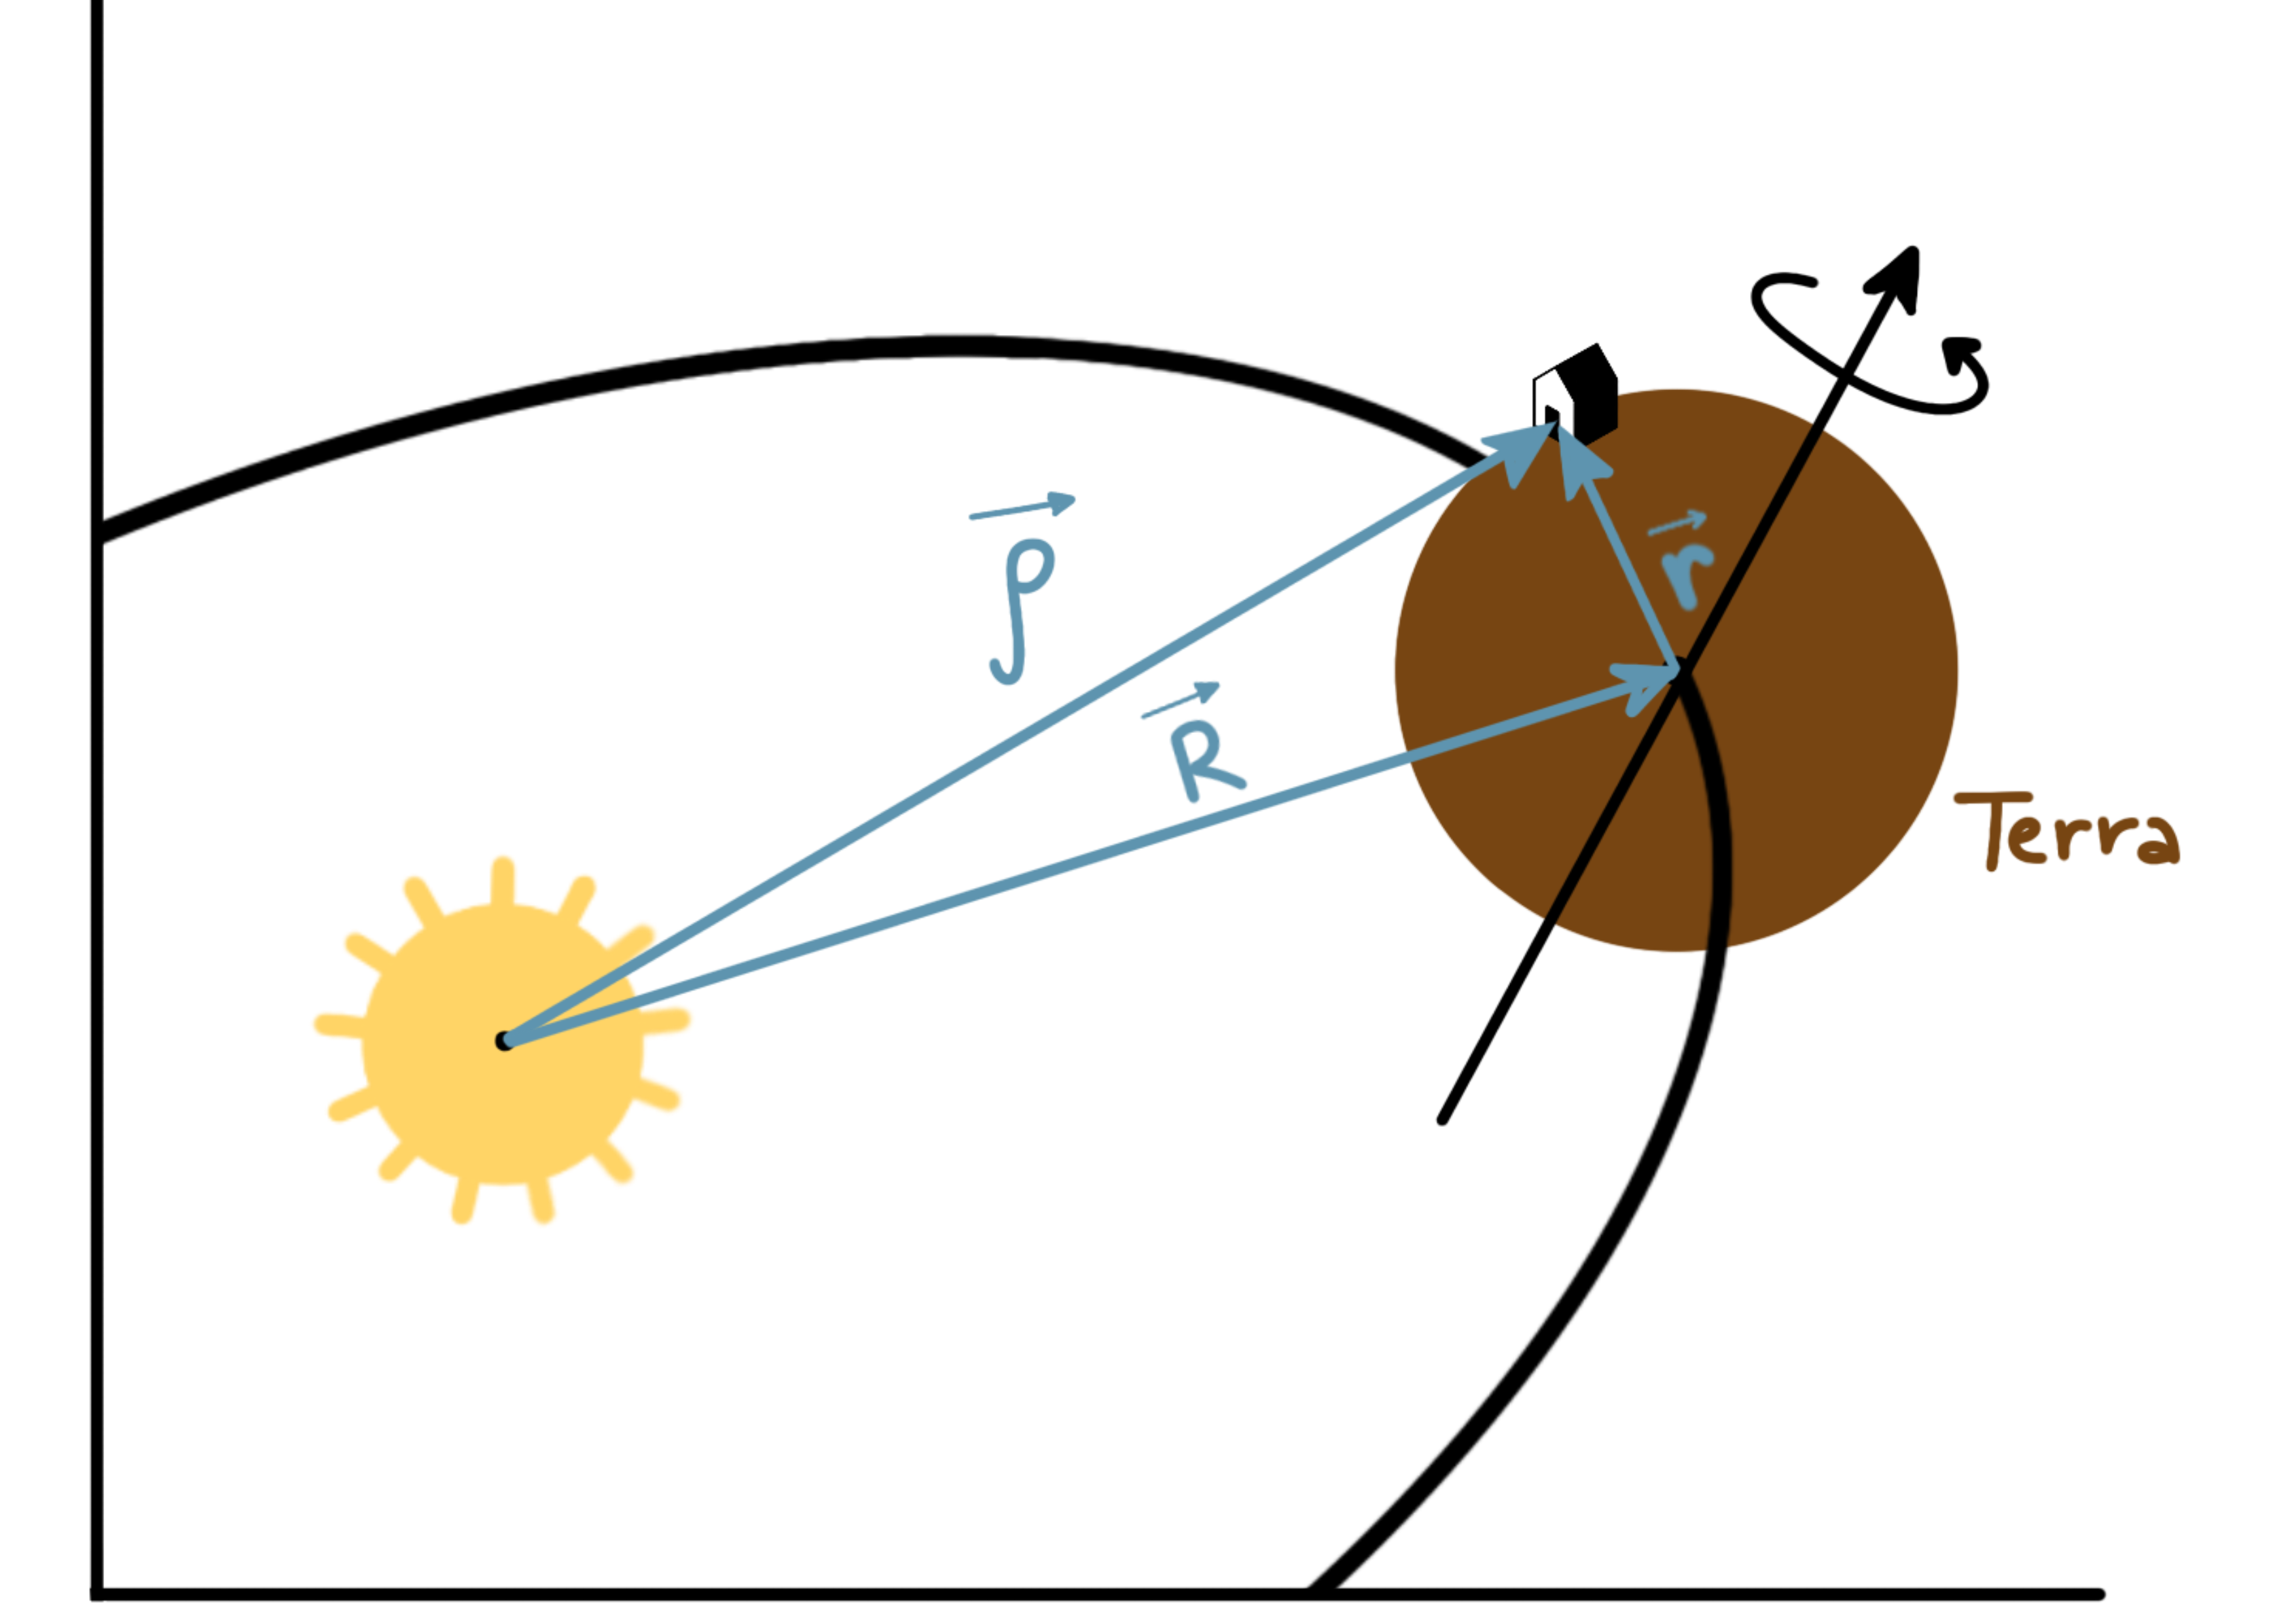
\includegraphics[width=\textwidth]{vectors.PNG}
        \caption{Els vectors que hem definit a la secció \ref{sec: seccio_2}.}
        \label{fig: sist_vectors}
    \end{subfigure}%
    \hspace{0.000001\textwidth}%
    \begin{subfigure}{0.5\textwidth}
        \centering
        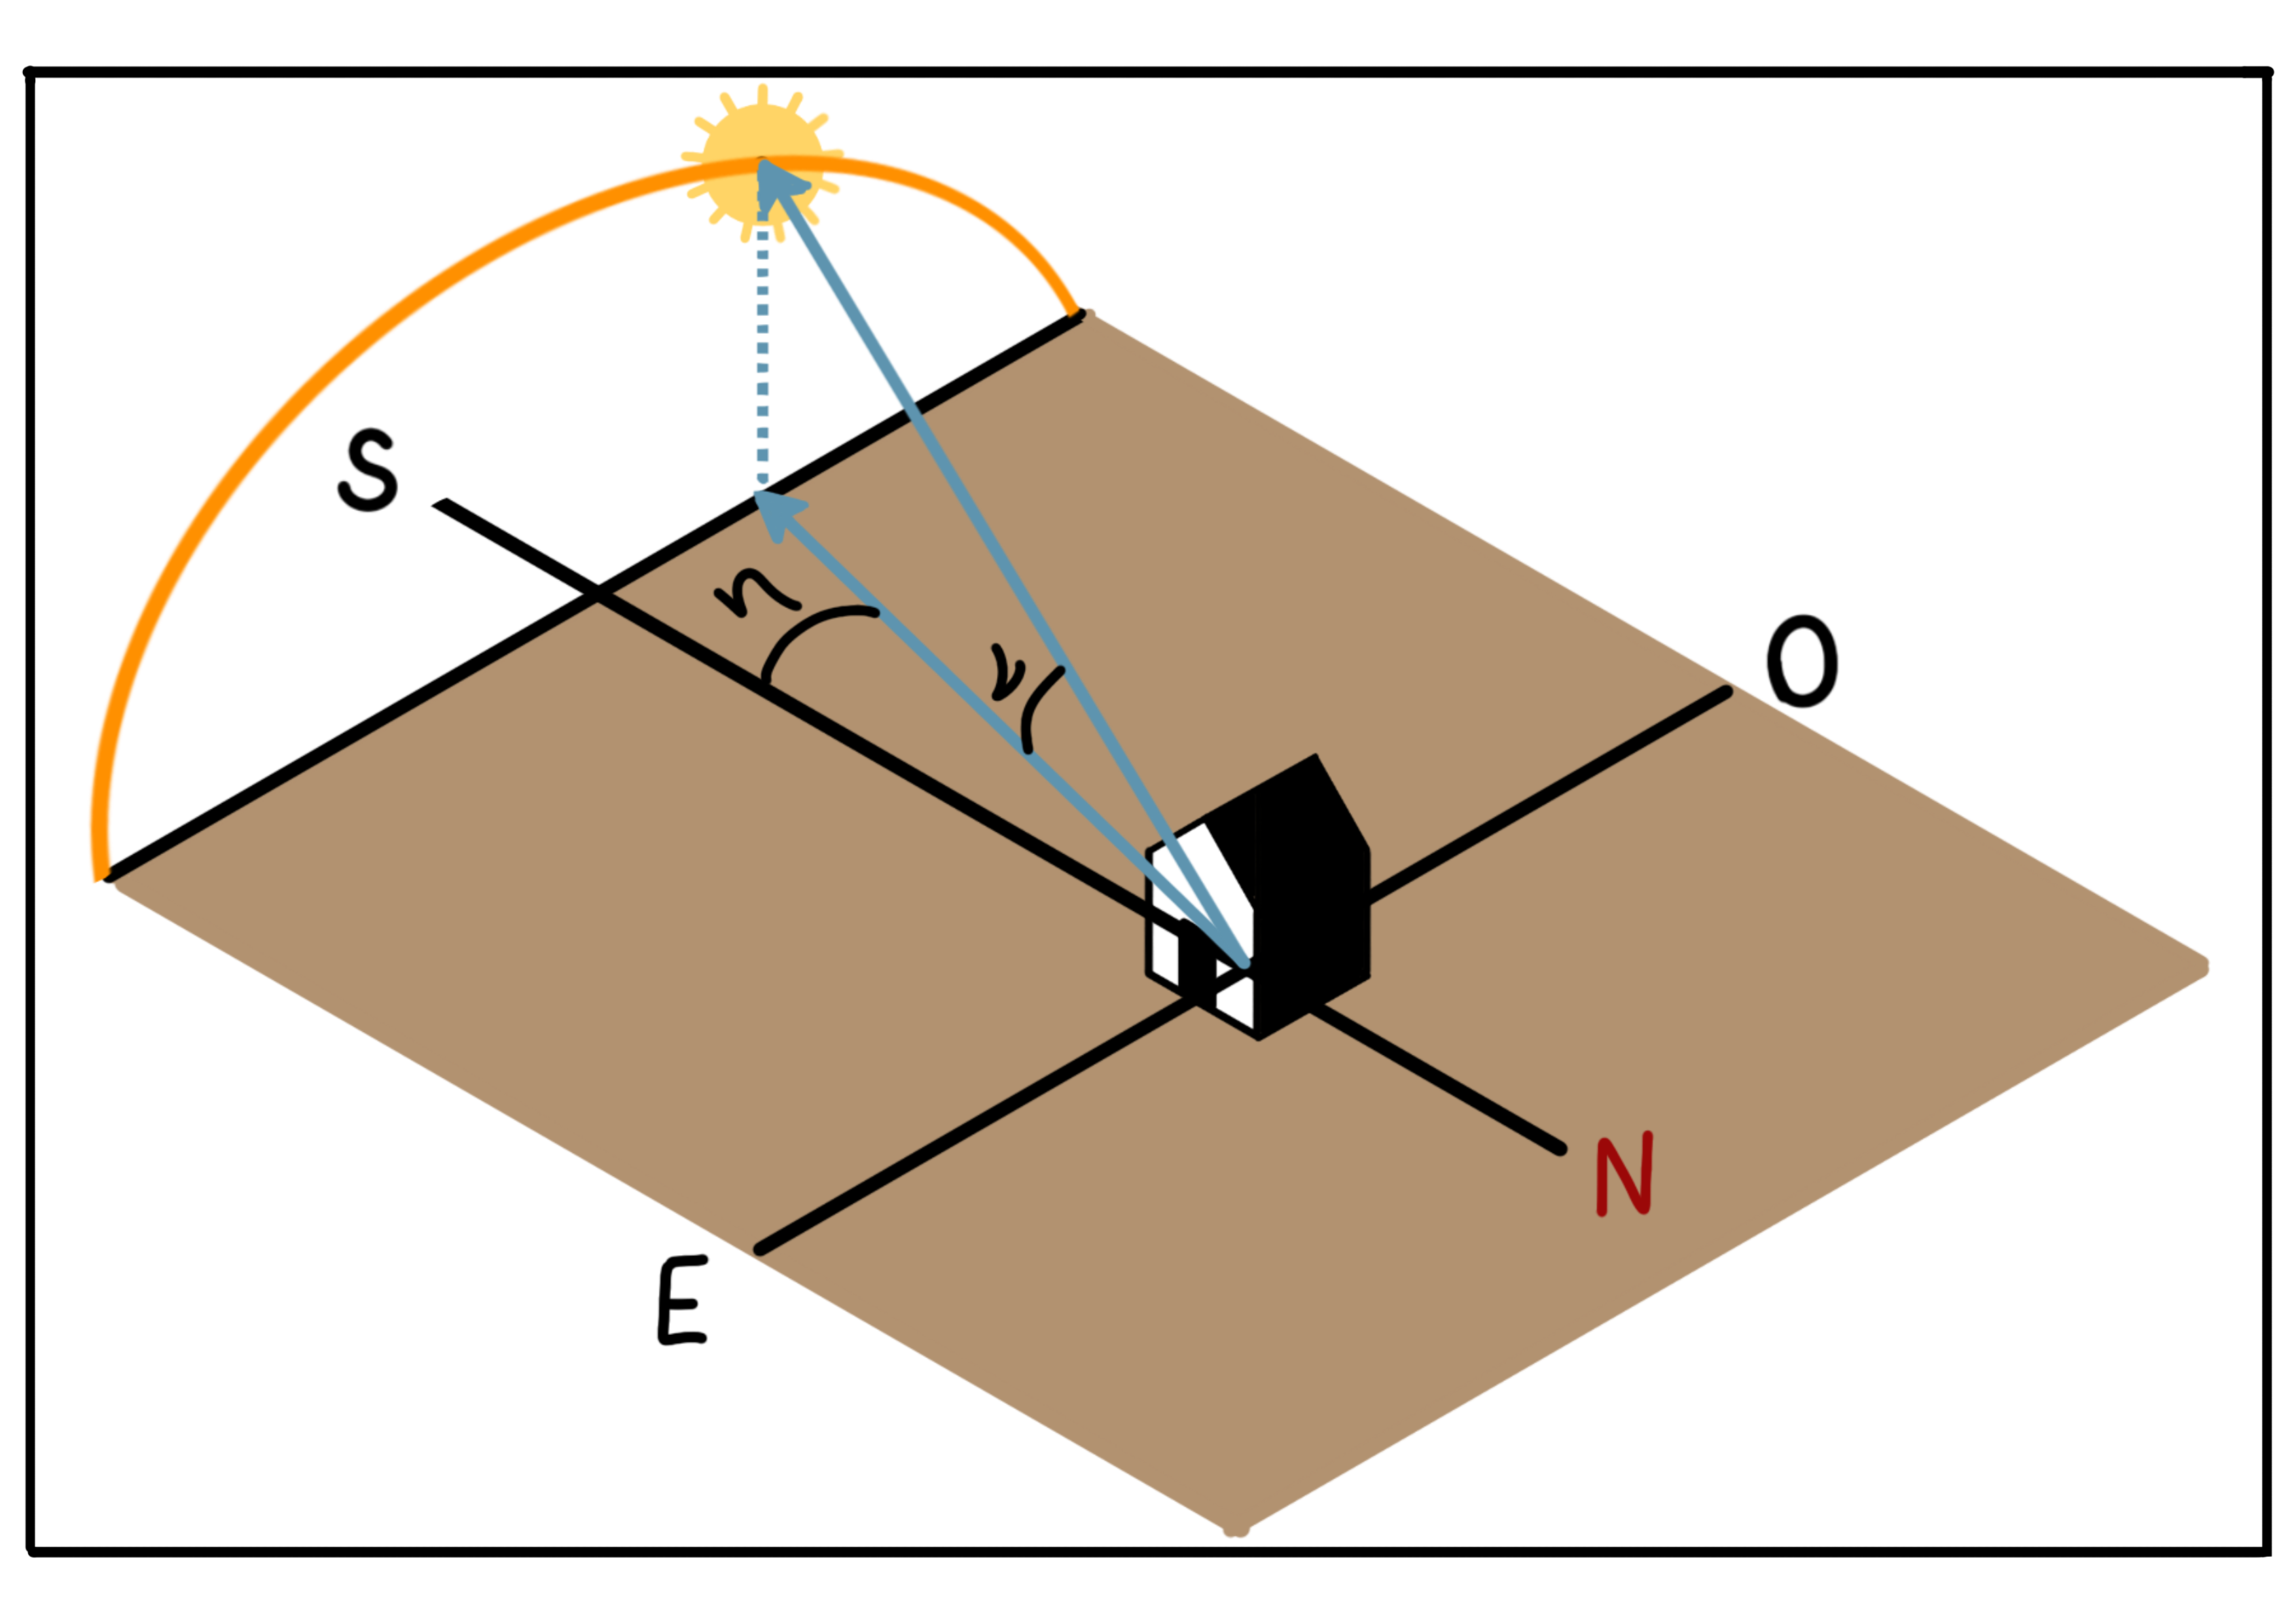
\includegraphics[width=\textwidth]{ang_sol.PNG}
        \caption{Els dos angles que hem usat per a determinar la posició del Sol.}
        \label{fig: sist_sol}
    \end{subfigure}
\end{figure}

També hem definit tres sistemes de referència (figura \ref{fig: sist_ref}) per facilitar els càlculs i trobar els àngles esmentats. Començant al sistema $\Omega$ podem obtenir un vector al sistema $\gamma$ a través de les matrius de rotació de l'annex \ref{annex: matr_rot}. Les relacions entre aquests sistemes són
\begin{itemize}
    \item Sistema $\Omega$: l'eix $z$ està orientat amb l'eix de rotació de la Terra.
    \item Sistema $\beta$: sistema rotat un angle $\beta$ en el pla $zy$ respecte el sistema $\Omega$. $\beta$ és l'angle entre l'eix de rotació de la terra i el vector perpendicular al pla de l'orbita, per tant, ara l'eix $z$ apunta en direcció pendicular al pla de l'òrbita.
    \item Sistema $\gamma$: sistema rotat un angle $\gamma$ en el pla $xy$ respecte el sistema $\beta$. $\gamma$ és l'angle entre $\vec{R}_{periheli}$ i $\vec{R}_{solstici(hivern)}$, per tant, ara la direcció de l'eix $y$ coincideix amb la direcció del periheli.
\end{itemize}
de tal manera que al sistema $\gamma$ tenim l'òrbita de la Terra amb el periheli i l'afeli sobre l'eix y i l'eix de rotació de la Terra orientat per tal que al solstici d'hivern (21 de Desembre) l'angle entre l'eix de rotació de la Terra i la direcció perpendicular al pla de l'òrbita sigui màxim.

Al sistema $\Omega$ el vector $\vec{r}$ és molt fàcil de definir 
\begin{equation}
    \vec{r}_{(t)}=r_T[\cos(\alpha)\cos(wt+\varphi)\hat{e_x}+\cos(\alpha)\sin(wt)+\varphi\hat{e_y}+\sin(\alpha)\hat{e_z}]
    \label{vector_r}
\end{equation}
si tenim la coordenada de latitud del punt de la Terra on volem fer els càlculs, $\alpha$, i el radi de la Terra, $r_T$, i on $w$ és la velocitat angular de rotació de la Terra i $t$ el temps transcorregut al llarg del dia.
Per tal de que aquest vector a $t=0$ comenci a la posició més allunyada del Sol (és a dir que t=0 es correspongui amb la meitat de la nit) hem d'afegir l'angle $\varphi$ a l'angle de rotació. $\varphi$ anirà variant cada dia i és l'angle entre el vector definit a (\ref{vector_r}) i el vector $\vec{R}$ a $t=0$.

El vector $\vec{R}$ ja el tenim calculat de la secció \ref{sec: seccio_1} i el vector $\vec{\rho}$ és simplement
\begin{equation}
    \vec{\rho}= \vec{R}+\vec{r}
\end{equation}
Un cop tenim aquests tres vectors els angles queden definits
\begin{equation}
    \nu=\angle (\vec{r}_{\gamma}, \vec{\rho}_{\gamma}) -\frac{\pi}{2}  
\end{equation}
\begin{equation}
    \eta=\pi - \angle (\vec{R}_{\Omega}, \vec{r}_{\Omega})
\end{equation}
on usem la funció arccosinus per trobar els angles.\footnote{$\angle (\vec{u}, \vec{v})= \arccos\left(\frac{\vec{u} \cdot \vec{v}}{\|\vec{u}\| \|\vec{v}\|}\right)$}


Si calculem aquests angles per una posició concreta a la Terra\footref{nota: habitatge}i pels dies que corresponen als equinocis i als solsticis obtenim el següent gràfic.
\begin{figure}[h]
    \centering
    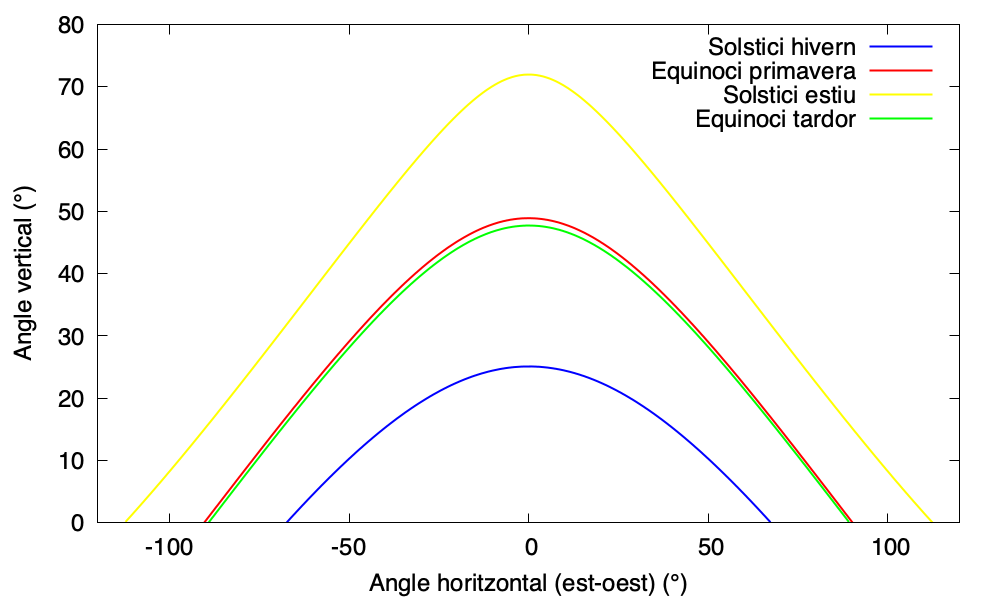
\includegraphics[width=0.5\textwidth]{equinocis.png}
    \label{solsticis}
    \caption{Angles del Sol al llarg d'un dia per diferents moments de l'any a un habitatge de Sant Cugat del Vallès}
\end{figure}

\section{Estudi de l'energia elèctrica}

\section{Resolució de l'EDO per diversos mètodes numèrics}\label{sec: edosRK}
Per a resoldre l'EDO de l'òrbita terrestre hem utilitzat el mètode d'Euler, però sabem que hi ha mètodes numèrics més potents que aquest. Per axò hem volgut comparar els resultats.

Els mètodes emprats per a resoldre l'equació \eqref{equ_en_r} han estat el Runge-Kutta d'ordre 2 i el Runge-Kutta d'ordre 4, amb la mateixa discretització temporal en els 3 mètodes numèrics.

\begin{figure}[hbt!]
    \centering
    \begin{subfigure}{0.5\textwidth}
        \centering
        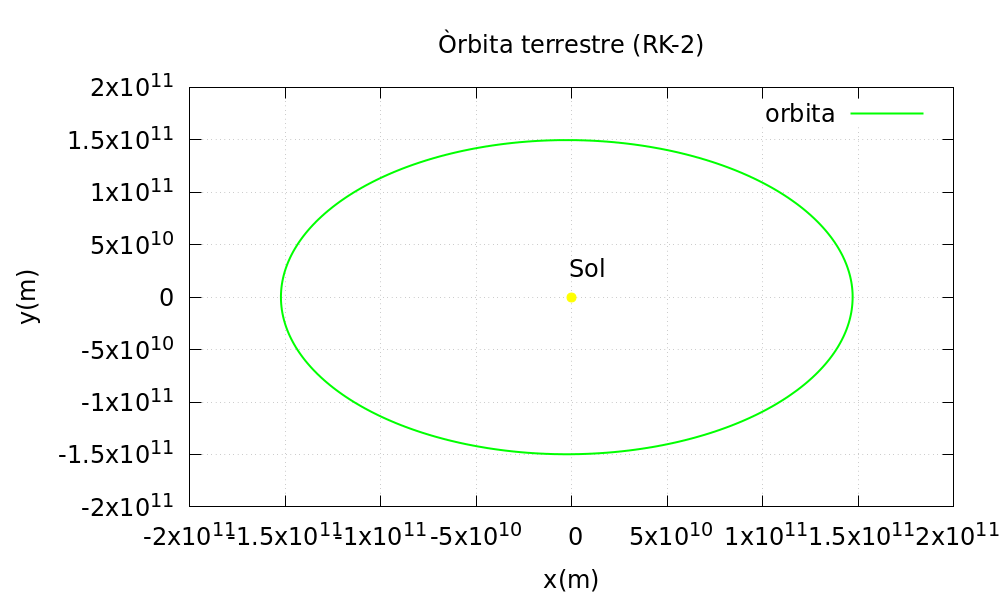
\includegraphics[width=\textwidth]{orbitaRK2.PNG}
        \caption{Òrbita terrestre per Runge-Kutta d'ordre 2}
        \label{fig: orbitaRK2}
    \end{subfigure}%
    \hspace{0.01\textwidth}%
    \begin{subfigure}{0.5\textwidth}
        \centering
        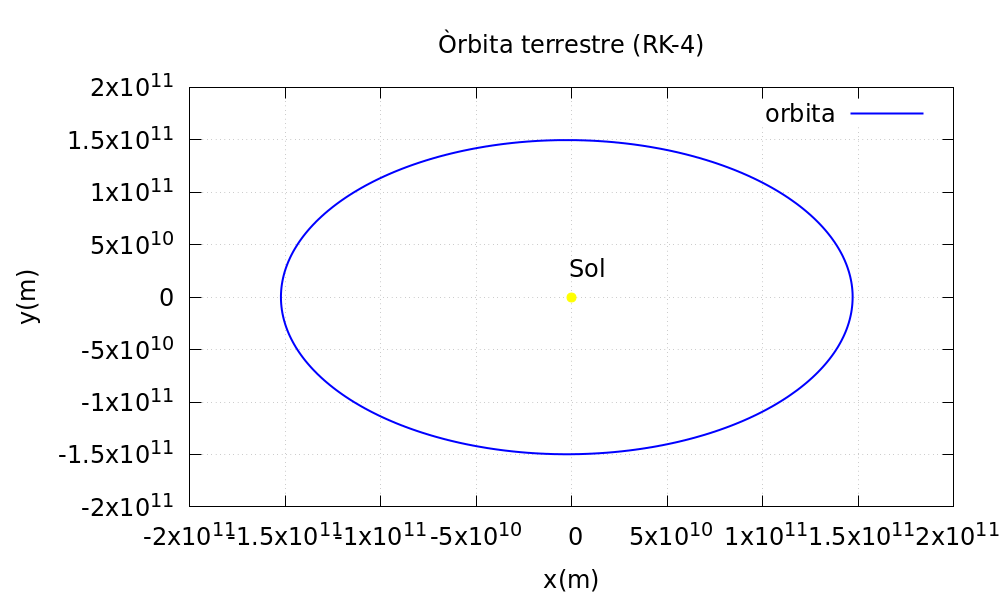
\includegraphics[width=\textwidth]{orbitaRK4.PNG}
        \caption{Òrbita terrestre per Runge-Kutta d'ordre 4}
        \label{fig: orbitaRK4}
    \end{subfigure}
        \hspace{0.01\textwidth}%
    \begin{subfigure}{0.5\textwidth}
        \centering
        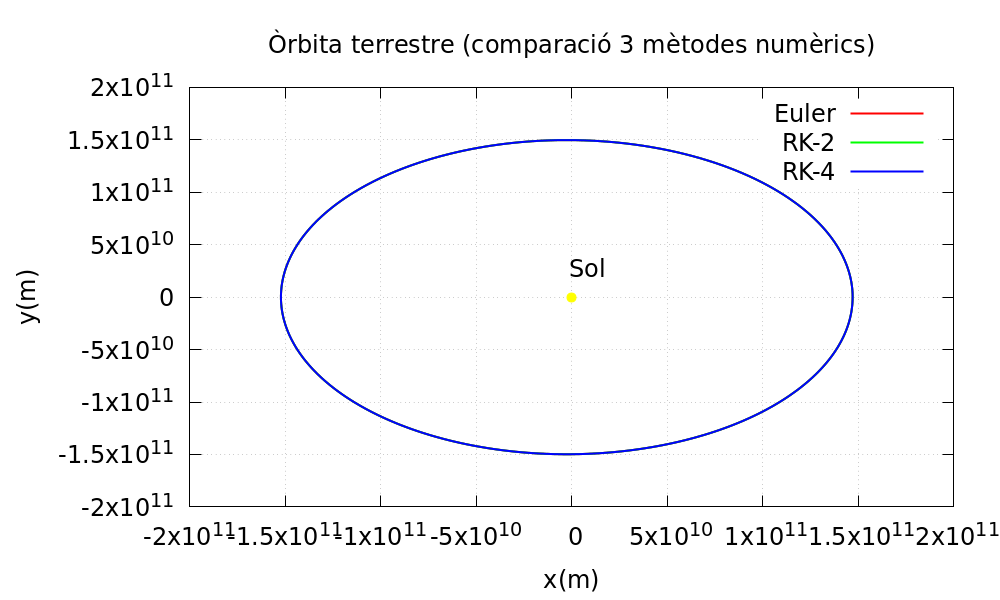
\includegraphics[width=\textwidth]{orbita3met.PNG}
        \caption{Òrbites terrestres per 3 mètodes numèrics}
        \label{fig: orbita3met}
    \end{subfigure}
\end{figure}

\section*{Annex}
\appendix

\section{Matrius de canvi de sistema de referència}\label{annex: matr_rot}
\begin{equation}
    \mathbf{R}_{\beta}=
    \begin{pmatrix}
      1 & 0 & 0   \\
      0 & \cos\beta& -sin\beta \\
      0 & sin\beta & cos\beta \\
    \end{pmatrix}
\end{equation}  

\begin{equation}
    \mathbf{R}_{\gamma}=
    \begin{pmatrix}
       \cos\beta& -sin\beta& 0 \\
       \sin\beta & cos\beta &0\\
      0 & 0 & 1  \\
    \end{pmatrix}
\end{equation}  


\section{Angles i vectors apartat 2}
\begin{figure}[hbt]
    \centering
    \begin{subfigure}{0.5\textwidth}
        \centering
        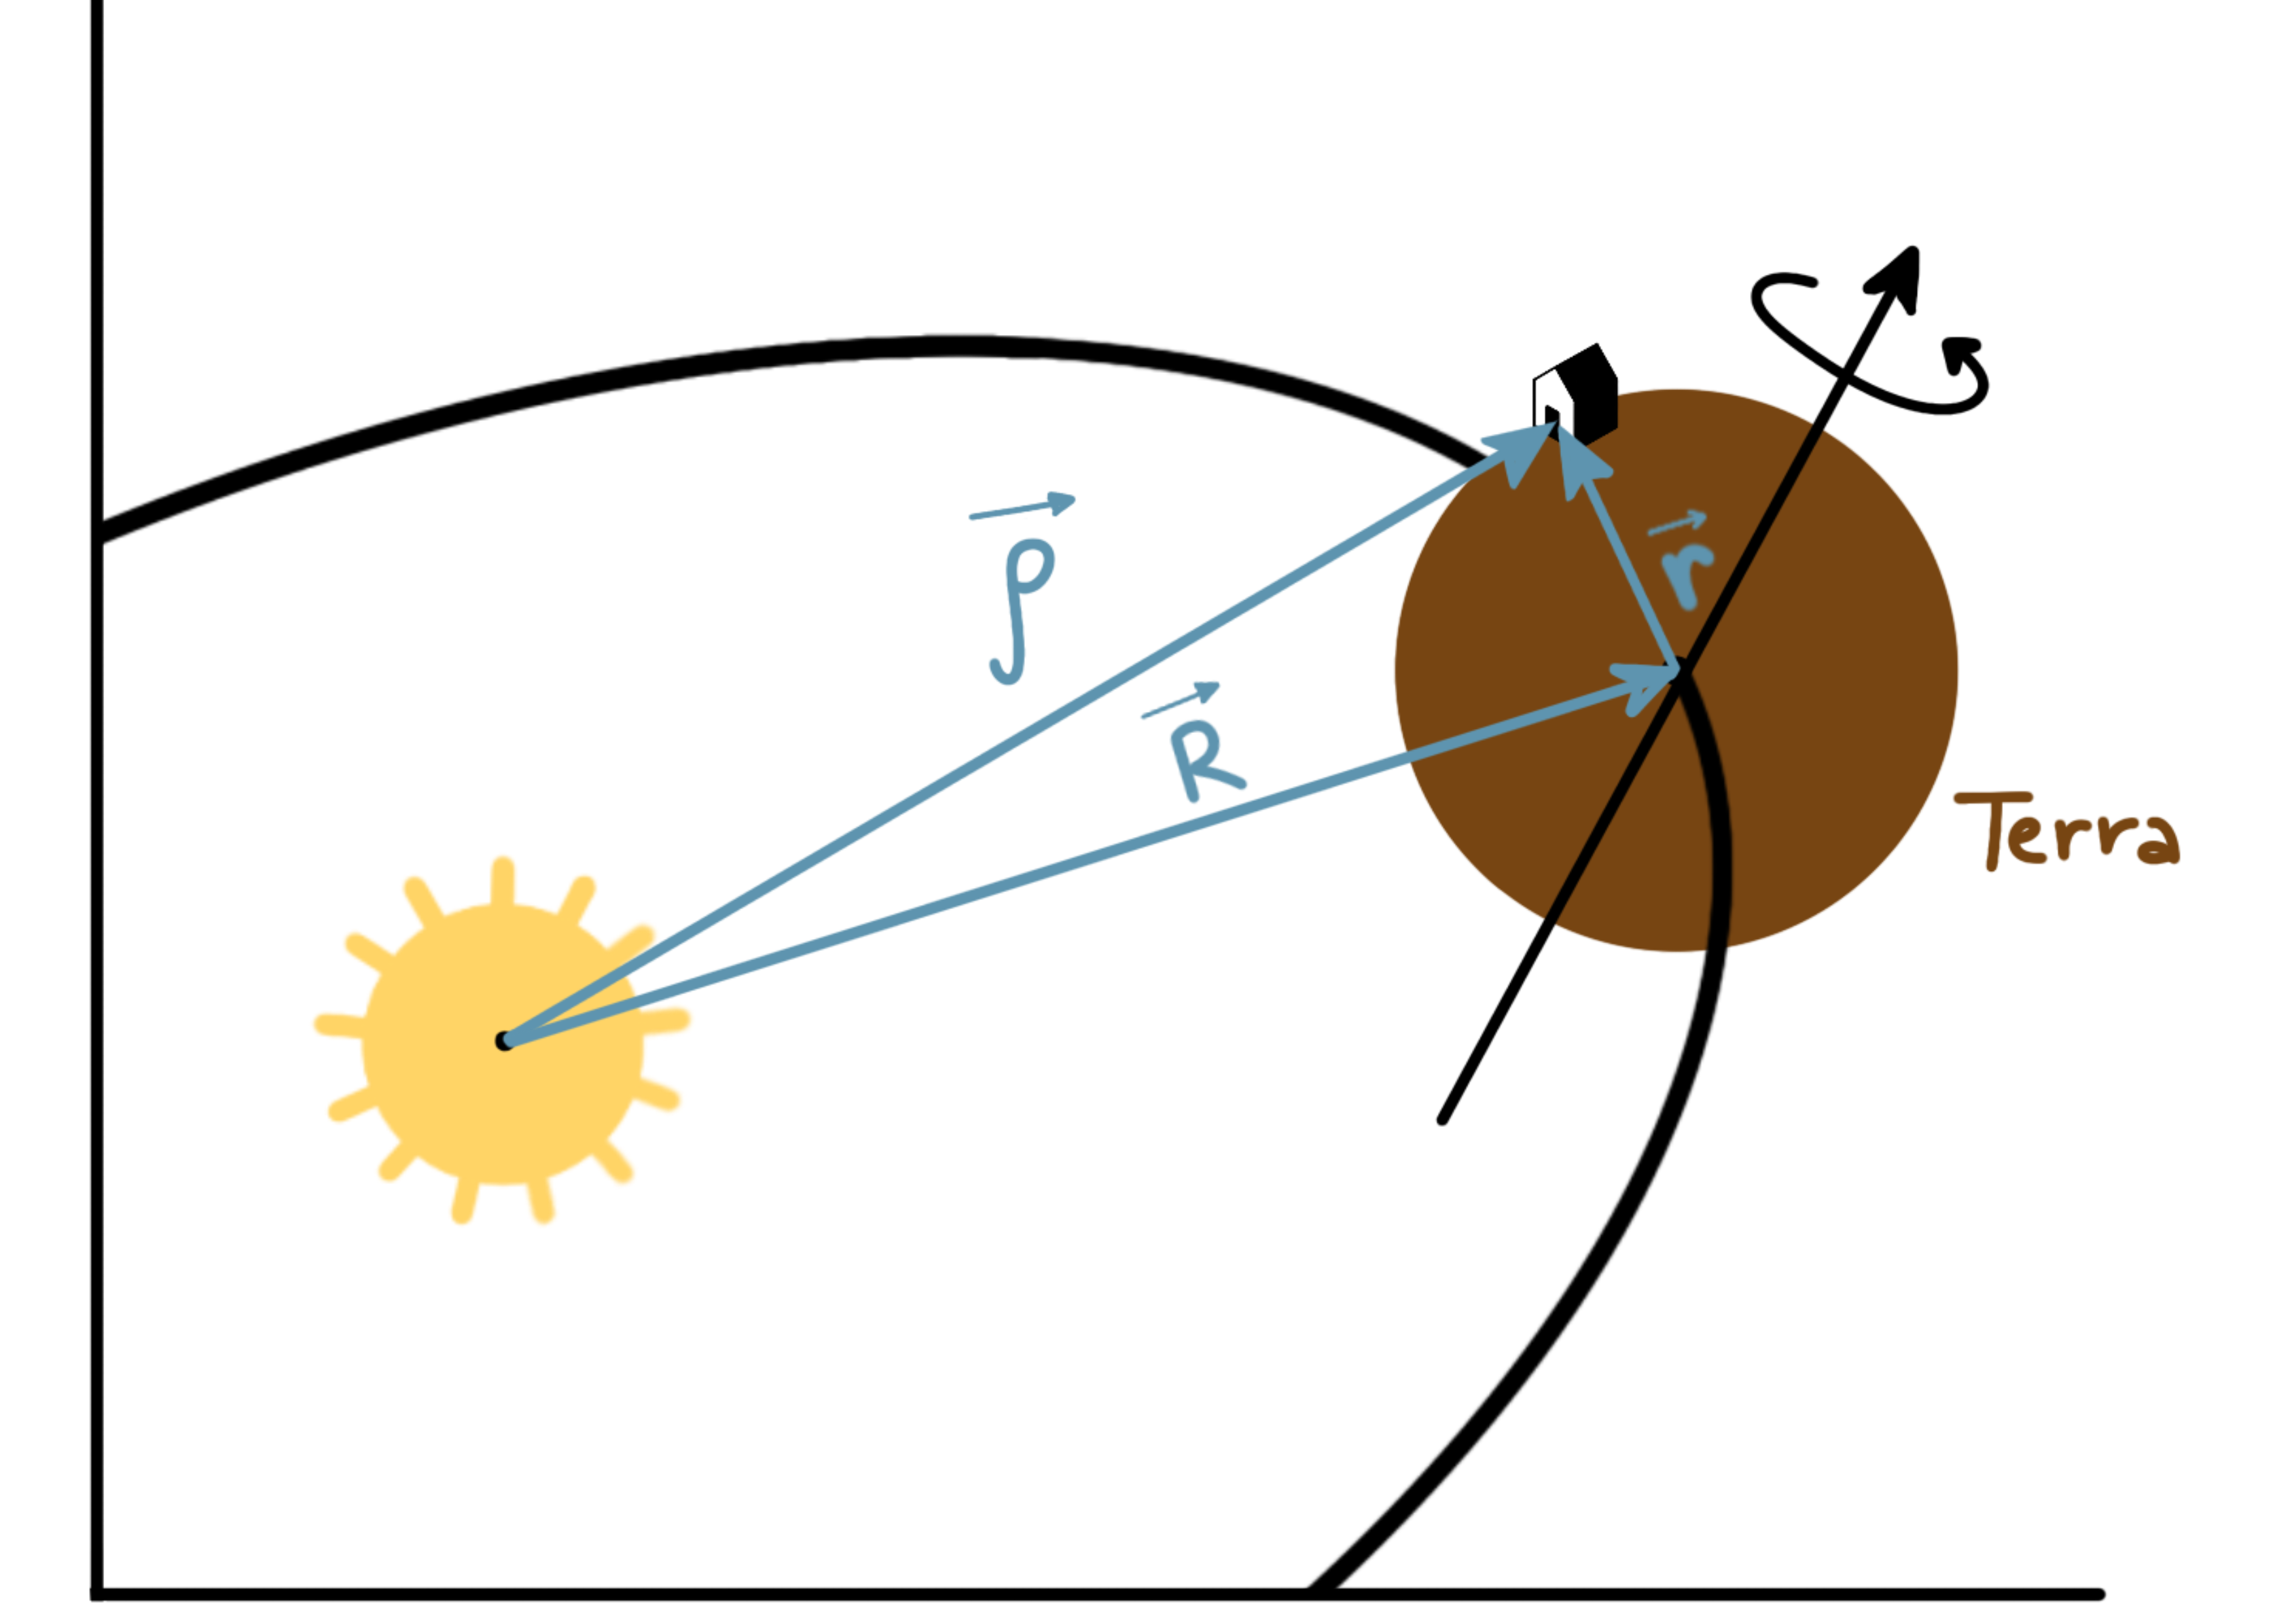
\includegraphics[width=\textwidth]{vectors.PNG}
        \caption{Els vectors que hem definit a la secció \ref{sec: seccio_2}.}
        \label{fig: sist_vectors}
    \end{subfigure}%
    \hspace{0.000001\textwidth}%
    \begin{subfigure}{0.5\textwidth}
        \centering
        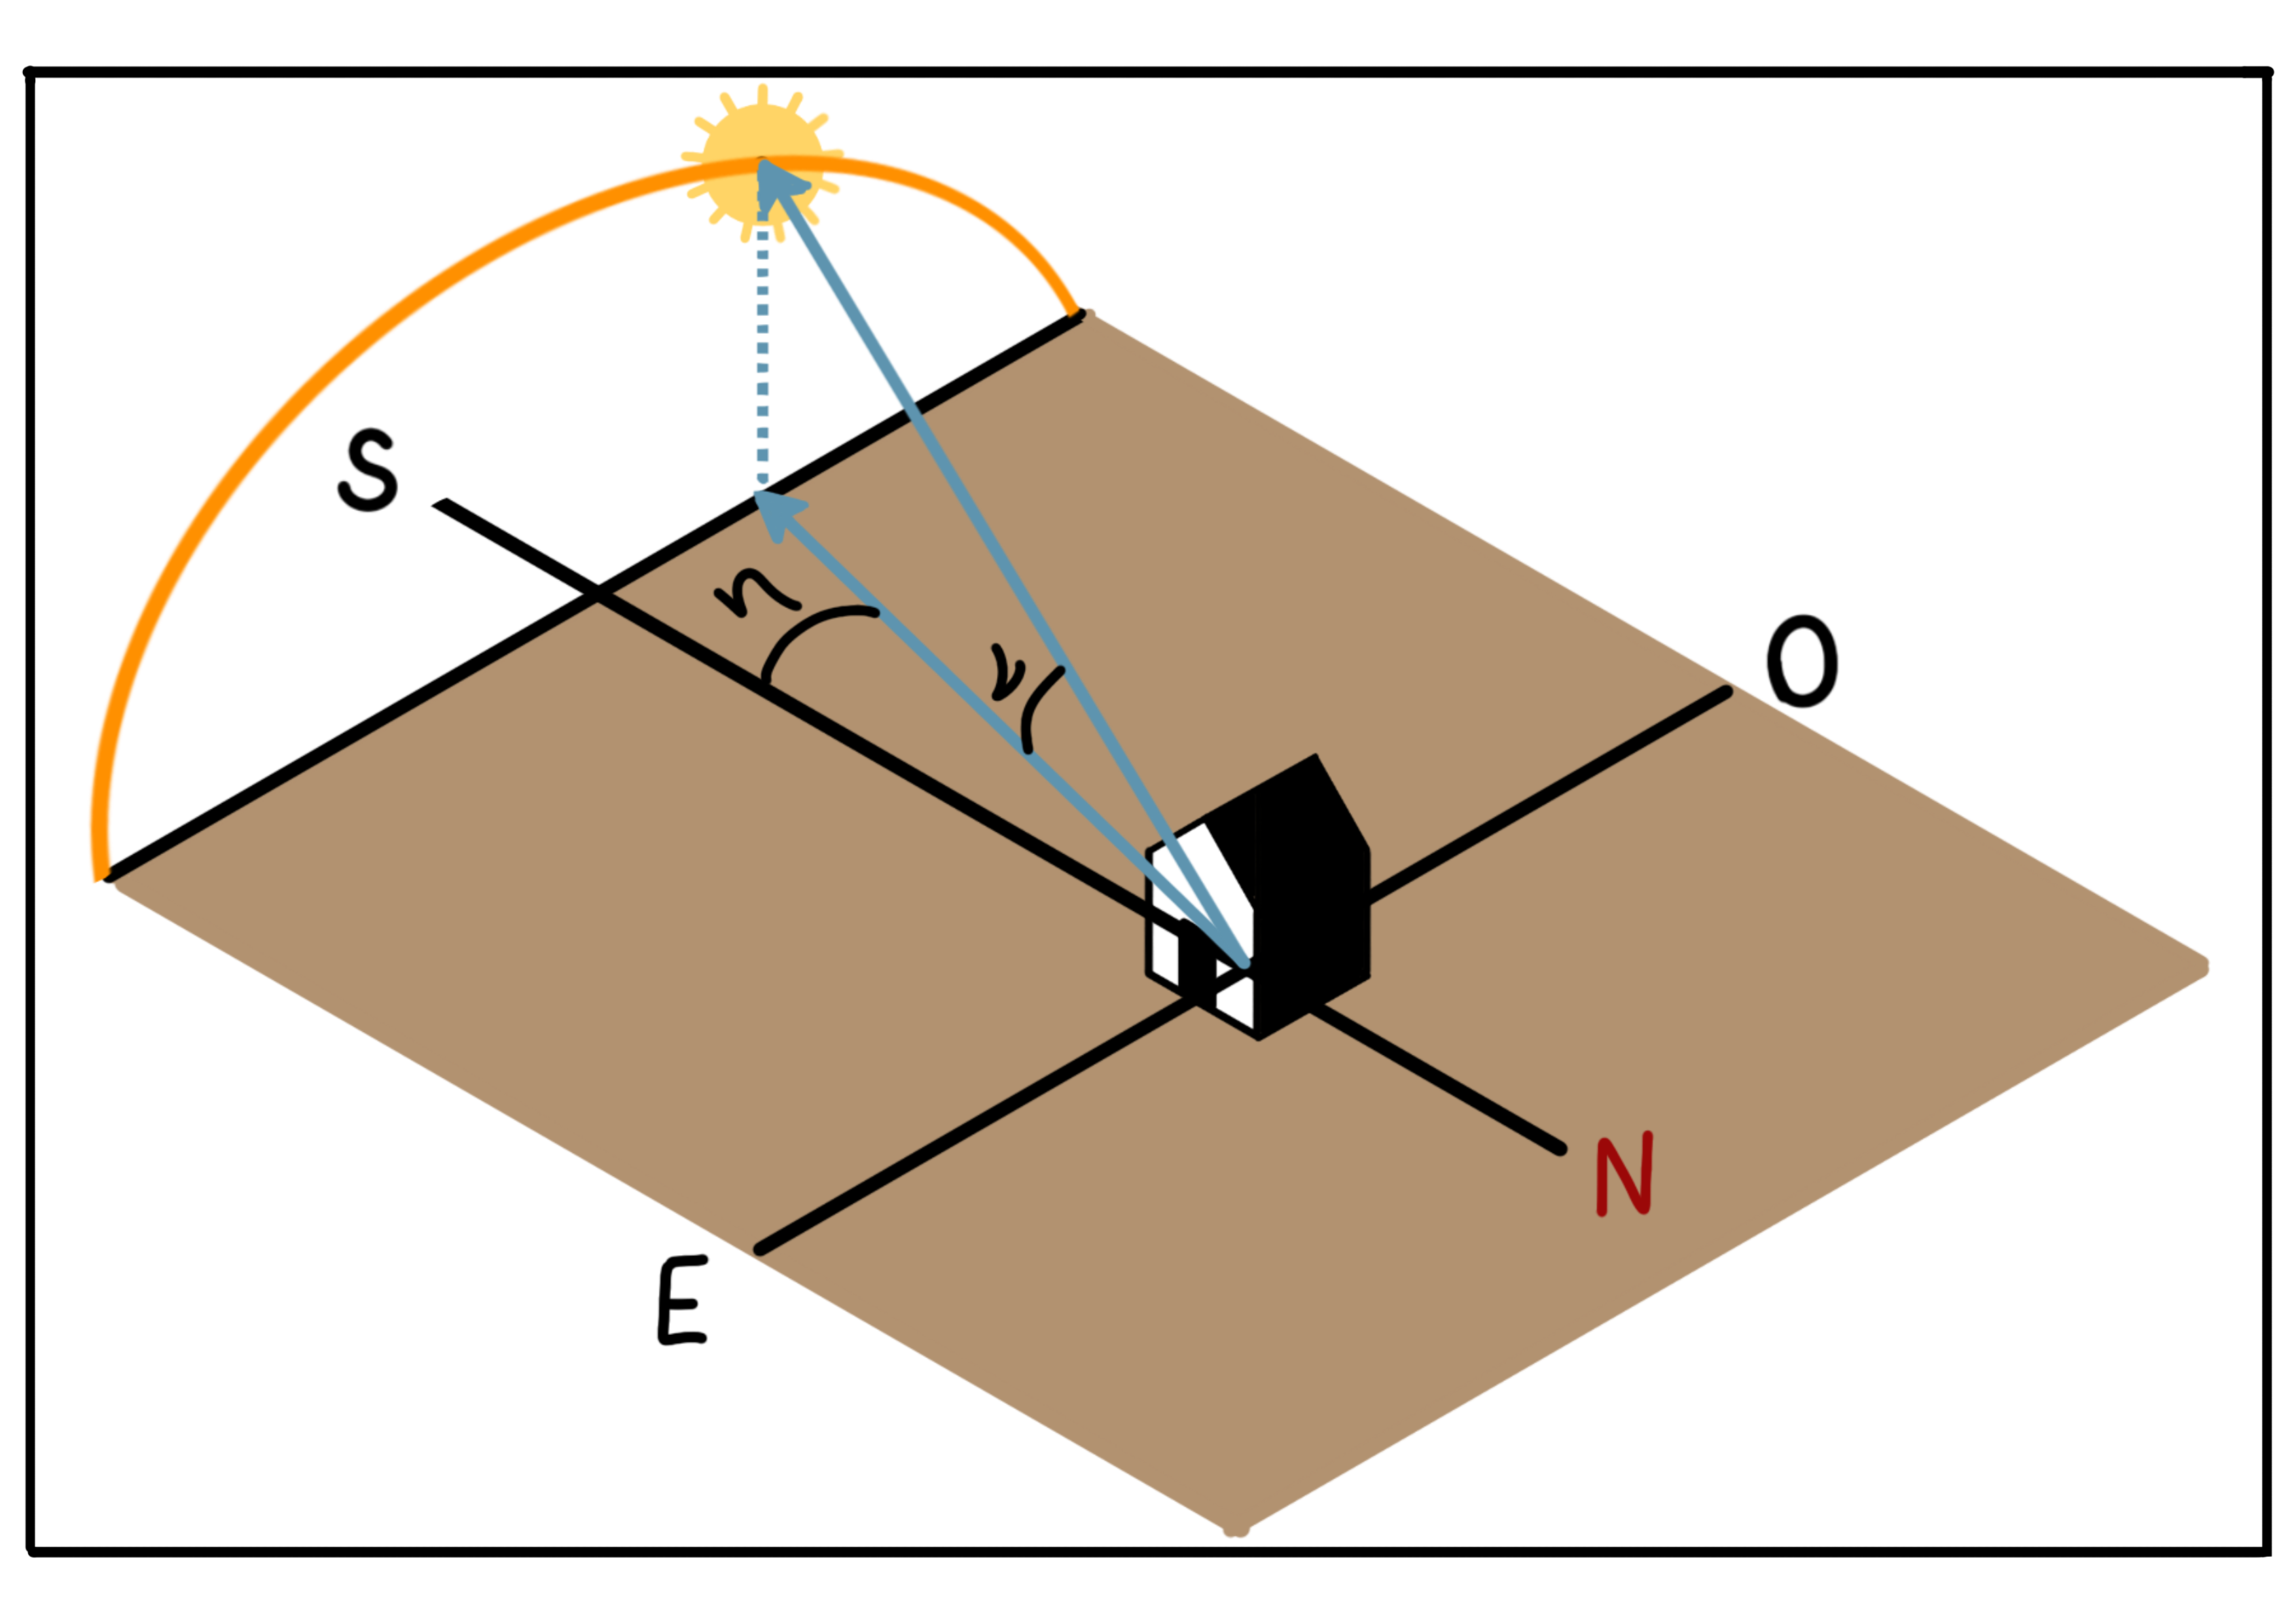
\includegraphics[width=\textwidth]{ang_sol.PNG}
        \caption{Els dos angles que hem usat per a determinar la posició del Sol.}
        \label{fig: sist_sol}
    \end{subfigure}
\end{figure}

\begin{figure}[hbt]
    \centering
    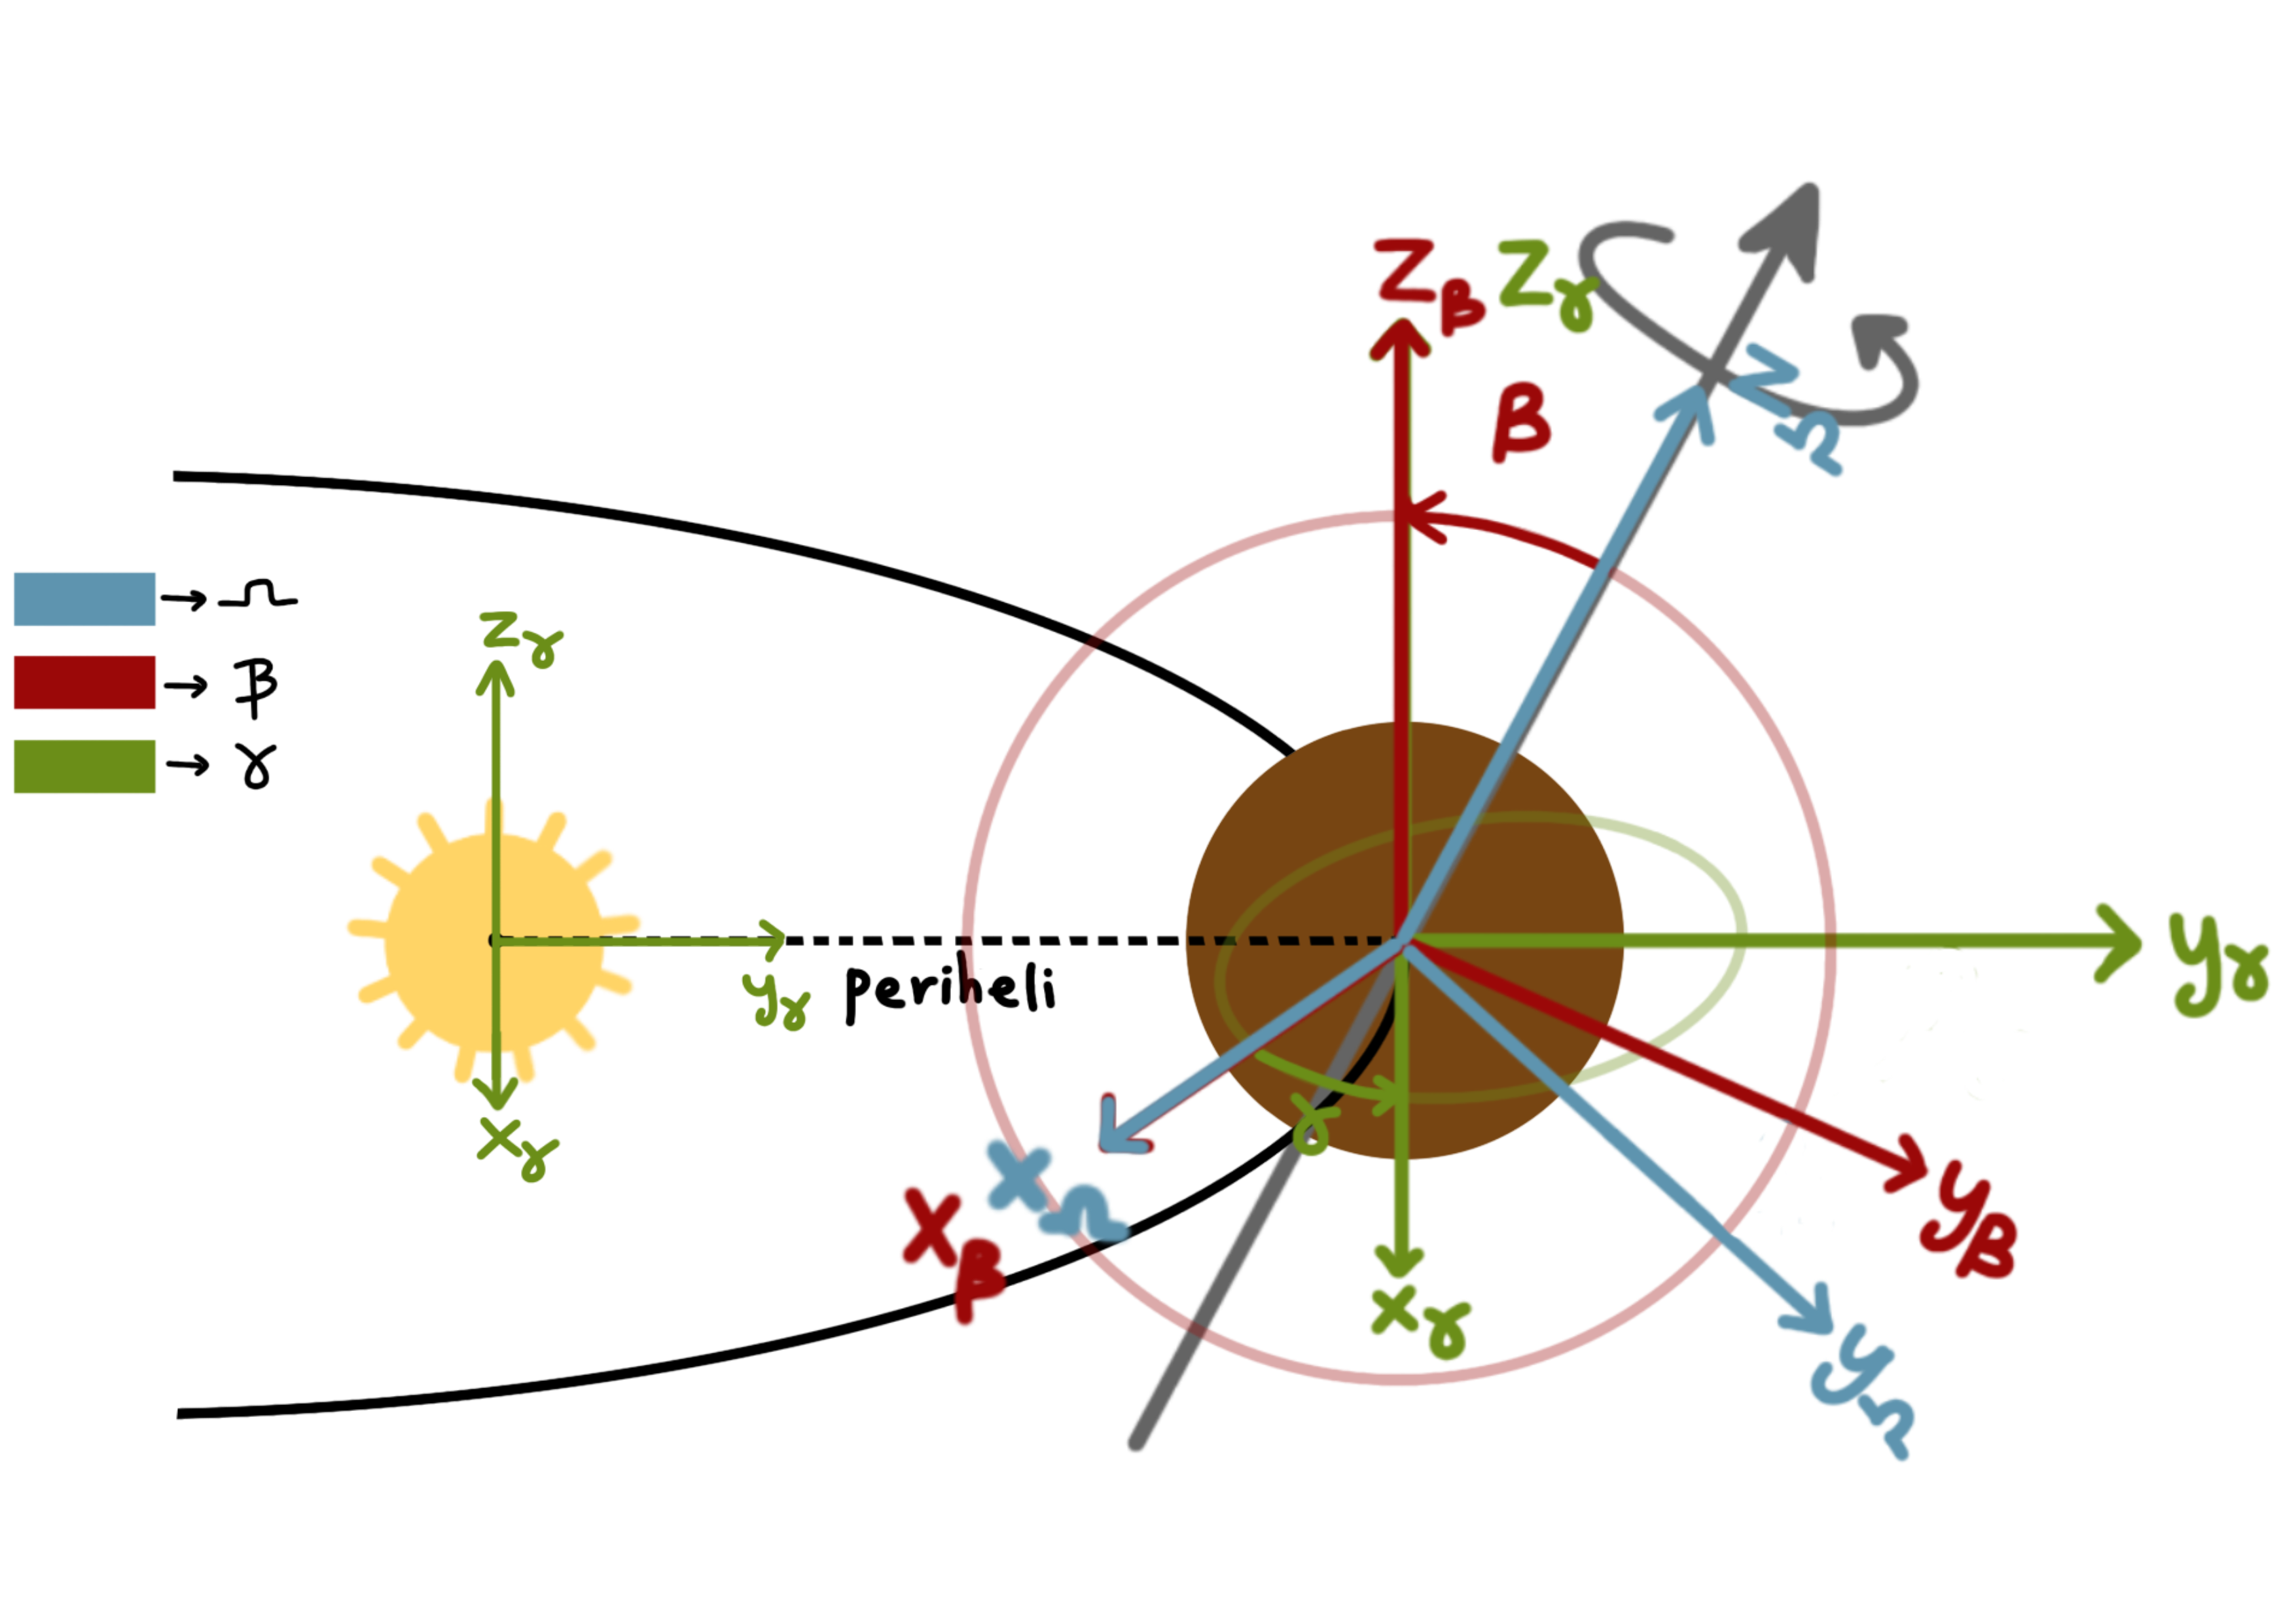
\includegraphics[width=0.5\textwidth]{sist_ref.PNG}
    \caption{Diferents sistemes de referència de la secció \ref{sec: seccio_2}.}
    \label{fig: sist_ref}
\end{figure}
\end{document}
